\begin{figure*}[!htbp]
  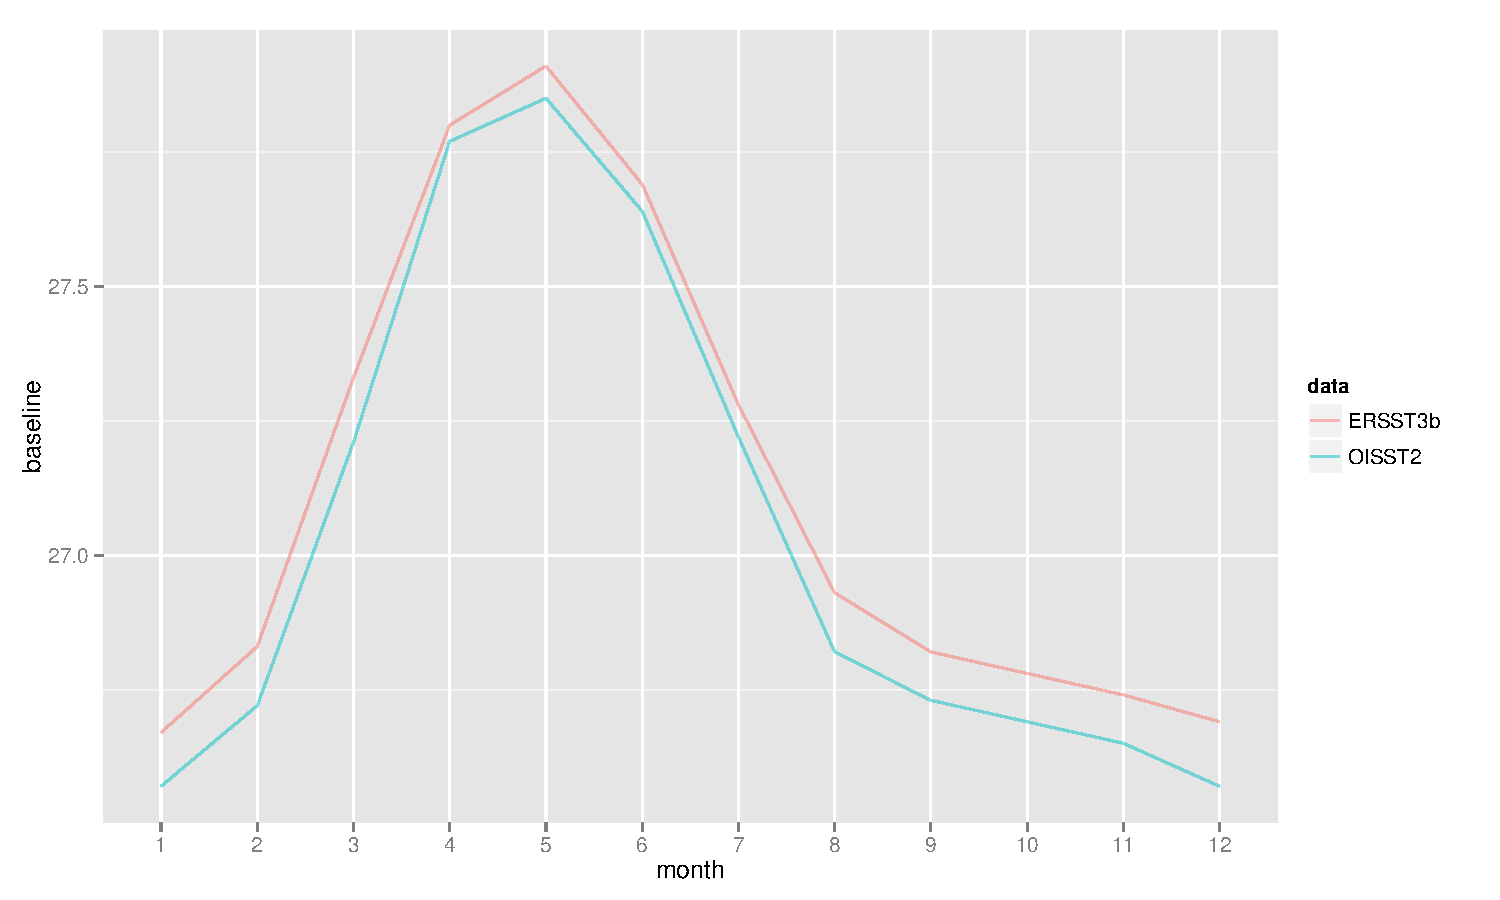
\includegraphics[width=\linewidth]{Pricingfigs/CompareOISSTandERRSTbaselines}
  \caption{Comparing OISST and ERSST monthly baselines}
   \label{fig:baeslinesOIER}
\end{figure*}

 Note OISSTs tendency toward colder SSTs. The cold bias in satellite data is a great concern in the climate literature and is noted in all the index construction papers on ERSST and OISST cited above.

Note also that February/March and June/July are inflection periods, moving both indexes from cold to warm phases (the former months) and back (the latter months). The baseline SST fluctuations over these two windows is dramatic. I suspect that those months will consequently host very active trading, if traded ENSO markets launch. Those are also likely to be the months where climate expertise and proprietary data will provide the largest edge to traders. The possibility of information asymmetries in those months may undermine the volume boost that traded markets might otherwise get from increased volatility. \index{sea-surface temperature!phases}



--------



With the exception of version 3 [footnote ERRST version 3 included infrared satellite data starting in 1985. NOAA determined that this addition introduced some bias into the index - it tended to suggest temperatures that were too cold by a factor of .01 deg C. NOAA consequently removed satellite data (although it retains in situ data collected via satellite) from the calculation of ERSST version 3b, the current standard.],
